\section{Overordnet arkitektur}
Den overordnede arkitekturskissen, figur \ref{fig:overordnet-ark}, 
beskriver den overordnede helheten i systemet. En sensor plasseres på 
hjul/nav på lastebilen. Denne sender vibrasjonsfrekvenssignaler til en 
prosesseringsenhet plassert sentralt i lastebilen. I prosesseringsenheten 
tolkes frekvenssignalet, og dersom det detekteres en anomalitet i 
frekvensområdet, rapporteres dette i et lesbart format opp til en 
smartskjerm montert i dashbordet i førerhuset på lastebilen.
\newline
\begin{figure}[H]
	\centering
	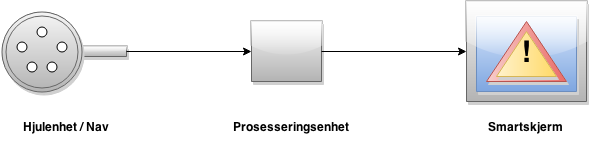
\includegraphics[width=1.00\textwidth]{images/arkitektur-overordnet.png}
	\label{fig:overordnet-ark}
	\caption{Overordnet arkitekturskisse.}
\end{figure}

Mer detaljert beskrivelse av arkitektur finnes i seksjon \ref{sec:arkitektur}
